\documentclass[11pt, a4paper]{article}
\usepackage[utf8x]{inputenc}
\usepackage[spanish]{babel}

\usepackage{graphicx}
\usepackage{float}
\usepackage[linktoc=all]{hyperref}

\usepackage{listings}
\usepackage{pxfonts}
\usepackage{xcolor}
\definecolor{deepblue}{rgb}{0,0,0.5}
\definecolor{deepred}{rgb}{0.6,0,0}
\definecolor{deepgreen}{rgb}{0,0.5,0}
\definecolor{backcolour}{rgb}{0.7,0.7,0.7}

\lstdefinestyle{mystyle}{
    backgroundcolor=\color{backcolour},   
    commentstyle=\color{deepgreen},
    keywordstyle=\bfseries\color{deepblue},
	otherkeywords={as, cv2, None},
    stringstyle=\color{deepgreen},
    basicstyle=\ttfamily\footnotesize,
    breakatwhitespace=false,         
    breaklines=true,                 
    captionpos=b,                    
    keepspaces=true,                 
    showspaces=false,                
    showstringspaces=false,
    showtabs=false,                  
    tabsize=4
}

\lstset{style=mystyle}
%------------------- Dimensiones -------------------
\usepackage{geometry}
\geometry{a4paper, total={170mm, 240mm}, top=20mm, left=20mm}
\setlength{\headheight}{15mm}% ...at least 51.60004pt
\setlength{\footskip}{15mm}% ...at least 51.60004pt
%----------------------------------------------------

%------------------- Encabezado y Pie de pág -------------------
\usepackage{fancyhdr}
\pagestyle{fancy}
\fancyhf{}
\lhead{Visión por computadora}
\rhead{TP11}
\rfoot{Página \thepage}
%----------------------------------------------------


%----------------------------- Documento -----------------------------------------------
\begin{document}
\begin{titlepage}
 \centering
	
\includegraphics[scale=0.80]{Imagenes/LOGO.jpg} \par
 	\vspace{1cm}
 	{\scshape\LARGE Universidad Tecnológica Nacional \par}
 	{\scshape\large Facultad Regional de Córdoba \par}
 	\vspace{1cm}
	{\bfseries \Large Trabajo Práctico De Laboratorio $N^{\circ} 11$\par}
 	\vspace{1.5cm}

	\begin{tabular}{ll}
		Lamas, Matías		&	65536 	\\
		Navarro, Facundo	&	63809
	\end{tabular}
	
	\vspace{1cm}
	Curso: 6r4 \\
	Grupo $N^{\circ} 5$
 	\vfill
	{\bfseries \LARGE Visión por computadora\par}
	{\bfseries \Large Alineación de imágenes usando SIFT\par}
	\vspace{1.5cm}
	Docentes: \par
	Ing. Araguás, Gastón \par
	Ing. Redolfi, Javier \par

 	\vfill
	{\large \today\par}
\end{titlepage}
	
	
\tableofcontents
\clearpage

	\section{Consigna}
	Considerando los pasos detallados a continuación, realizar una alineación entre imágenes utilizando el algoritmo de SIFT.
	\begin{itemize}\itemsep 0em
		\item Capturar dos imágenes con diferentes vistas del mismo objeto.
		\item Computar puntos de interés y descriptores en ambas imágenes.
		\item Establecer matches entre ambos conjuntos de descriptores.
		\item Eliminar matches usando criterio de \textit{Lowe}.
		\item Computar una homografía entre un conjunto de puntos y el otro.
		\item Aplicar la homografía sobre una de las imágenes y guardarla en otra (mezclarla con un alpha de 50\%).
	\end{itemize}

	\section{Desarrollo}
	Importamos las librerias a usar, opencv y numpy.
	\lstinputlisting[language=python, firstline=3, lastline=4]{AlineacionSIFT.py}

	Cargamos el par de imágenes a utilizar, y guardamos unas copias de las mismas para dibujar sobre ellas los puntos claves (\textit{keypoints o kp}).
	\lstinputlisting[language=Python, firstline=8, lastline=11]{AlineacionSIFT.py}

	Para utilizar una instancia del detector de puntos claves \textit{SIFT}, hay que llamar a la función \textcolor{orange}{\textbf{\textit{cv2.xfeatures2d.SIFT.create()}}}. Todos los argumentos de la función tienen valores predeterminados, los cuales son:

	\begin{figure}[H]
		\centering
		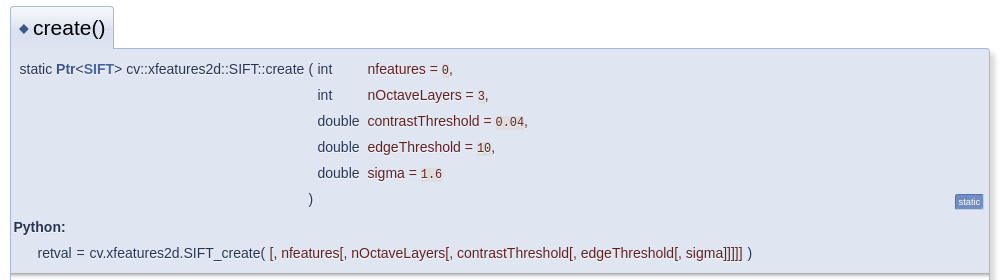
\includegraphics[width=0.8\textwidth]{Imagenes/sift_fn.png}
		\caption{Función create() del descriptor SIFT.}
		\label{fig:sift_fn}
	\end{figure} 
	
	En ese orden indican, el número de puntos claves a encontrar y retornar, número de niveles en la escala piramidal a usar, dos límites para ajustar la sensibilidad del algoritmo, la variación sigma para pre filtrar la imagen. Sin restarle importancia al resto de los argumentos, probablemente el más importante sea el primero para determinar la cantidad de puntos claves a buscar seguido por el sigma. Este último controla el tamaño máximo de los objetos que no son de interés, y es útil a la hora de remover el ruido o detalles innecesarios de la imagen. 
	
	\lstinputlisting[language=Python, firstline=13, lastline=15]{AlineacionSIFT.py}

	Luego dibujamos los puntos encontrados en cada imagen, el resultado se puede ver en la imagen \textcolor{blue}{\textbf{\ref{fig:sift_kp}}}.
	\lstinputlisting[language=Python, firstline=17, lastline=18]{AlineacionSIFT.py}

	\begin{figure}[H]
		\centering
		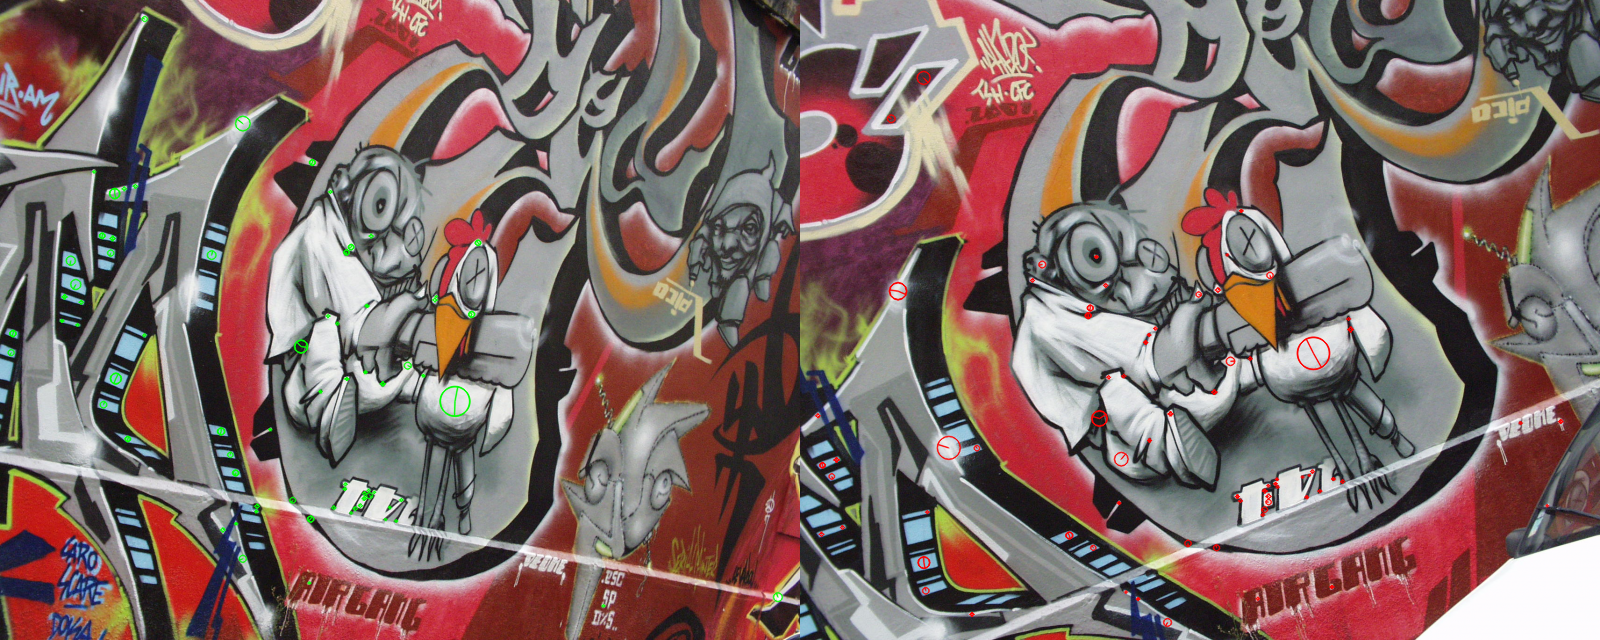
\includegraphics[width=\textwidth]{Imagenes/sift_kp.png}
		\caption{Imágenes con puntos claves encontrados por SIFT.}
		\label{fig:sift_kp}
	\end{figure} 

	Una vez encontrados los puntos claves por los descriptores, procedemos a encontrar las correspondencias entre ellos, opencv provee una gran variedad de herramientas para esto, el método más obvio y simple es el de comparar todos los posibles pares y elegir los mejores. Hay que destacar que este método es extremadamente lento. 

	Usamos la función \textcolor{orange}{\textbf{\textit{cv2.BFMatcher\_create()}}}, el cual toma una bandera que configura una distancia para la comparación entre descriptores y habilita la bandera de chequeo cruzado.

	\lstinputlisting[language=Python, firstline=26, lastline=26]{AlineacionSIFT.py}

		Una vez encontrada las correlaciones, se filtran los resultados de dos maneras distintas. Primero a través del método del vecino mas cercano (\textit{knn}), al cual se le aplica una comprobación del radio, comprueba dos radios entre el primer y segundo elemento, si es mayor a 0.8 (criterio de \textit{Lowe} = 0.7) se descarta, esto permite eliminar cerca del 90\% de falsas correspondencias, mientras que descarta solo el 5\% de correspondencias correctas.

	\lstinputlisting[language=Python, firstline=28, lastline=42]{AlineacionSIFT.py}

	El segundo filtrado se hace comprobando si las correspondencias encontradas en \textit{img2} para los puntos claves en \textit{img1} son los mismo encontrados en \textit{img1} para los puntos claves en \textit{img2}, es decir que solo conservamos las correspondencias encontradas en ambas direcciones.
	
	\lstinputlisting[language=Python, firstline=44, lastline=45]{AlineacionSIFT.py}
	
	\begin{figure}[H]
		\centering
		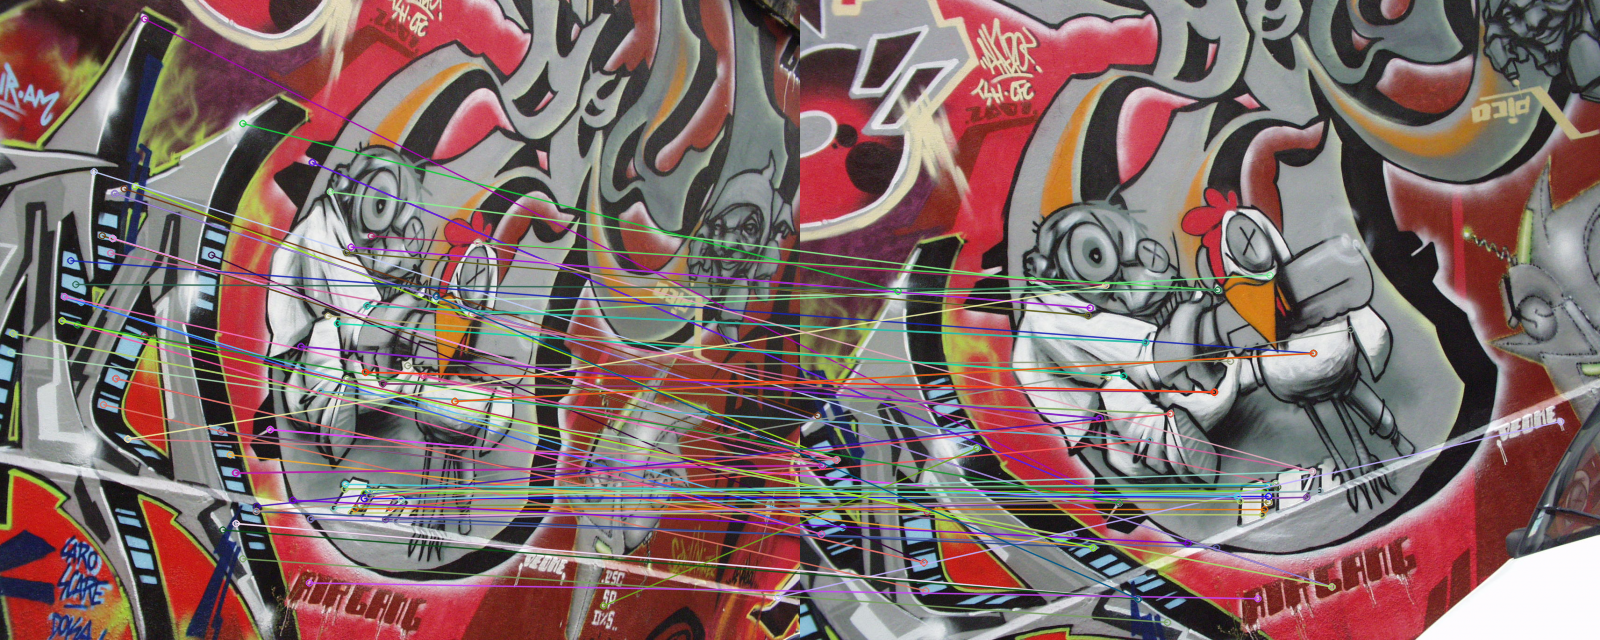
\includegraphics[width=\textwidth]{Imagenes/sift_mtch_nf.png}
		\caption{Correspondencias entre las imágenes sin filtrar.}
		\label{fig:sift_mtch_nf}
	\end{figure} 
	
	\begin{figure}[H]
		\centering
		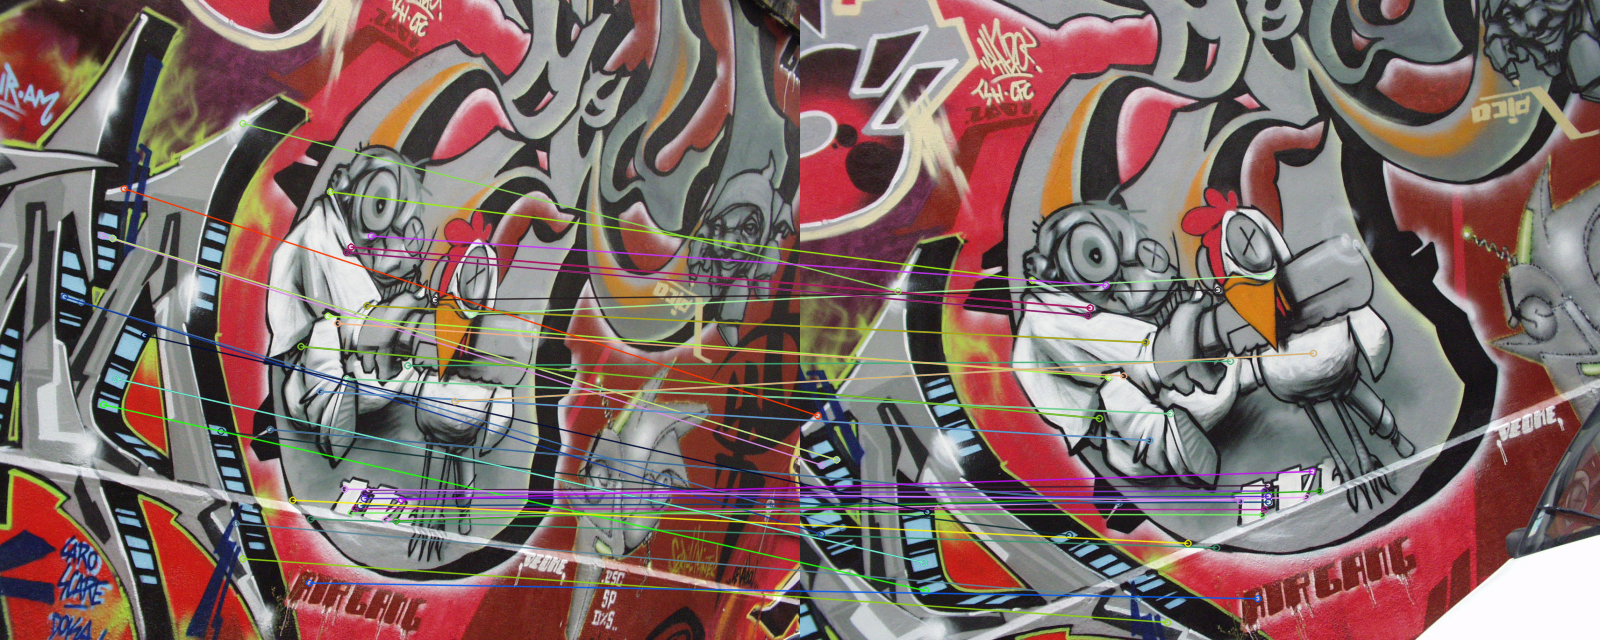
\includegraphics[width=\textwidth]{Imagenes/sift_mtch.png}
		\caption{Correspondencias entre las imágenes luego de filtrado}
		\label{fig:sift_mtch}
	\end{figure} 
	
	El siguiente paso es calcular la matriz homográfica entre las dos imágenes utilizando el algoritmo de \textit{RANSAC} (\textit{RANdom SAmple Consensus}), a través de la función \textcolor{orange}{\textbf{cv2.findHomography()}}, una vez que conseguimos la matriz, aplicamos la transformación perspectiva sobre una de las imágenes.

	\lstinputlisting[language=Python, firstline=62, lastline=69]{AlineacionSIFT.py}

	Finalmente, ponderamos la imagen a la cual le aplicamos la transformación a un valor ``alpha" y la otra imagen con su complemento y las unimos, dando como resultado la imagen que se muestra en \textcolor{blue}{\textbf{\ref{fig:sift_out}}}
	
	\begin{figure}[H]
		\centering
		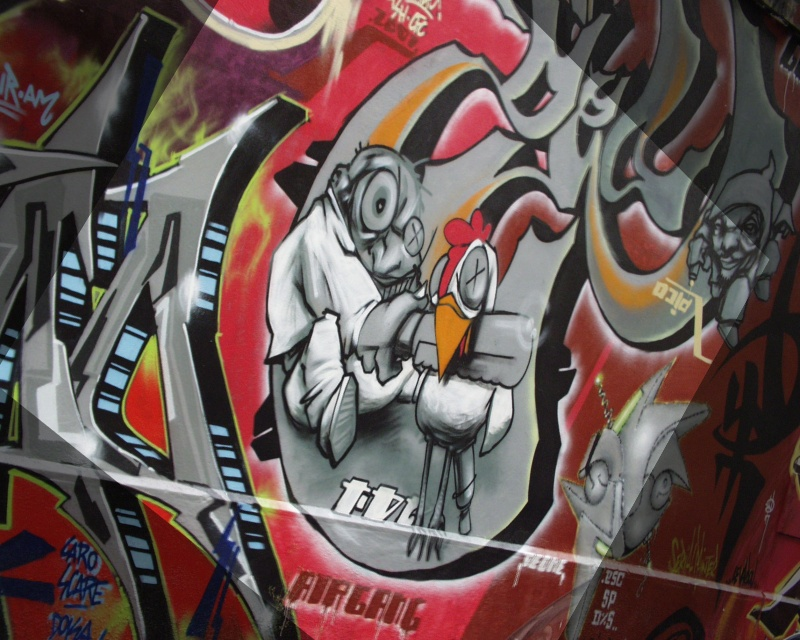
\includegraphics[width=\textwidth]{Imagenes/sift_out.png}
		\caption{Resultado final de aplicar el descriptor SIFT y aplicar la transformación homográfica.}
		\label{fig:sift_out}
	\end{figure} 

	\begin{thebibliography}{0}
		\bibitem{}  OpenCV 3 Computer Vision with Python Cookbook 
		\bibitem{}  Introduction to SIFT (Scale-Invariant Feature Transform) [OpenCV-Python Tutorials]
	\end{thebibliography}
\end{document}
